\section{Versuchsaufbau}
Für die folgenden Versuche werden folgende Bauteile auf unterschiedlichen Weisen miteinander verbunden und eingestellt. Es wird ein analoges Oszilloskop, in diesem Fall ein HAMEG HM-205-3(\ref{fig:oszilloskop}), ein Frequenzgenerator, hier ein HAMEG HM8030-4(\ref{fig:frequenzgenerator}), sowie ein Gerät, welches einen elektrischen Schwingkreis enthält benötigt. Letzteres Gerät setzt sich aus zwei festensowie einem variablen ohmschen Widerstand, einer Spule L und einem Kondensator C zusammen(\ref{fig:geraet2}). Weiterhin wird ein Tastkopf benötigt.
\begin{figure}[H]
    \centering

    \begin{subfigure}{0.45\textwidth}
        \centering
        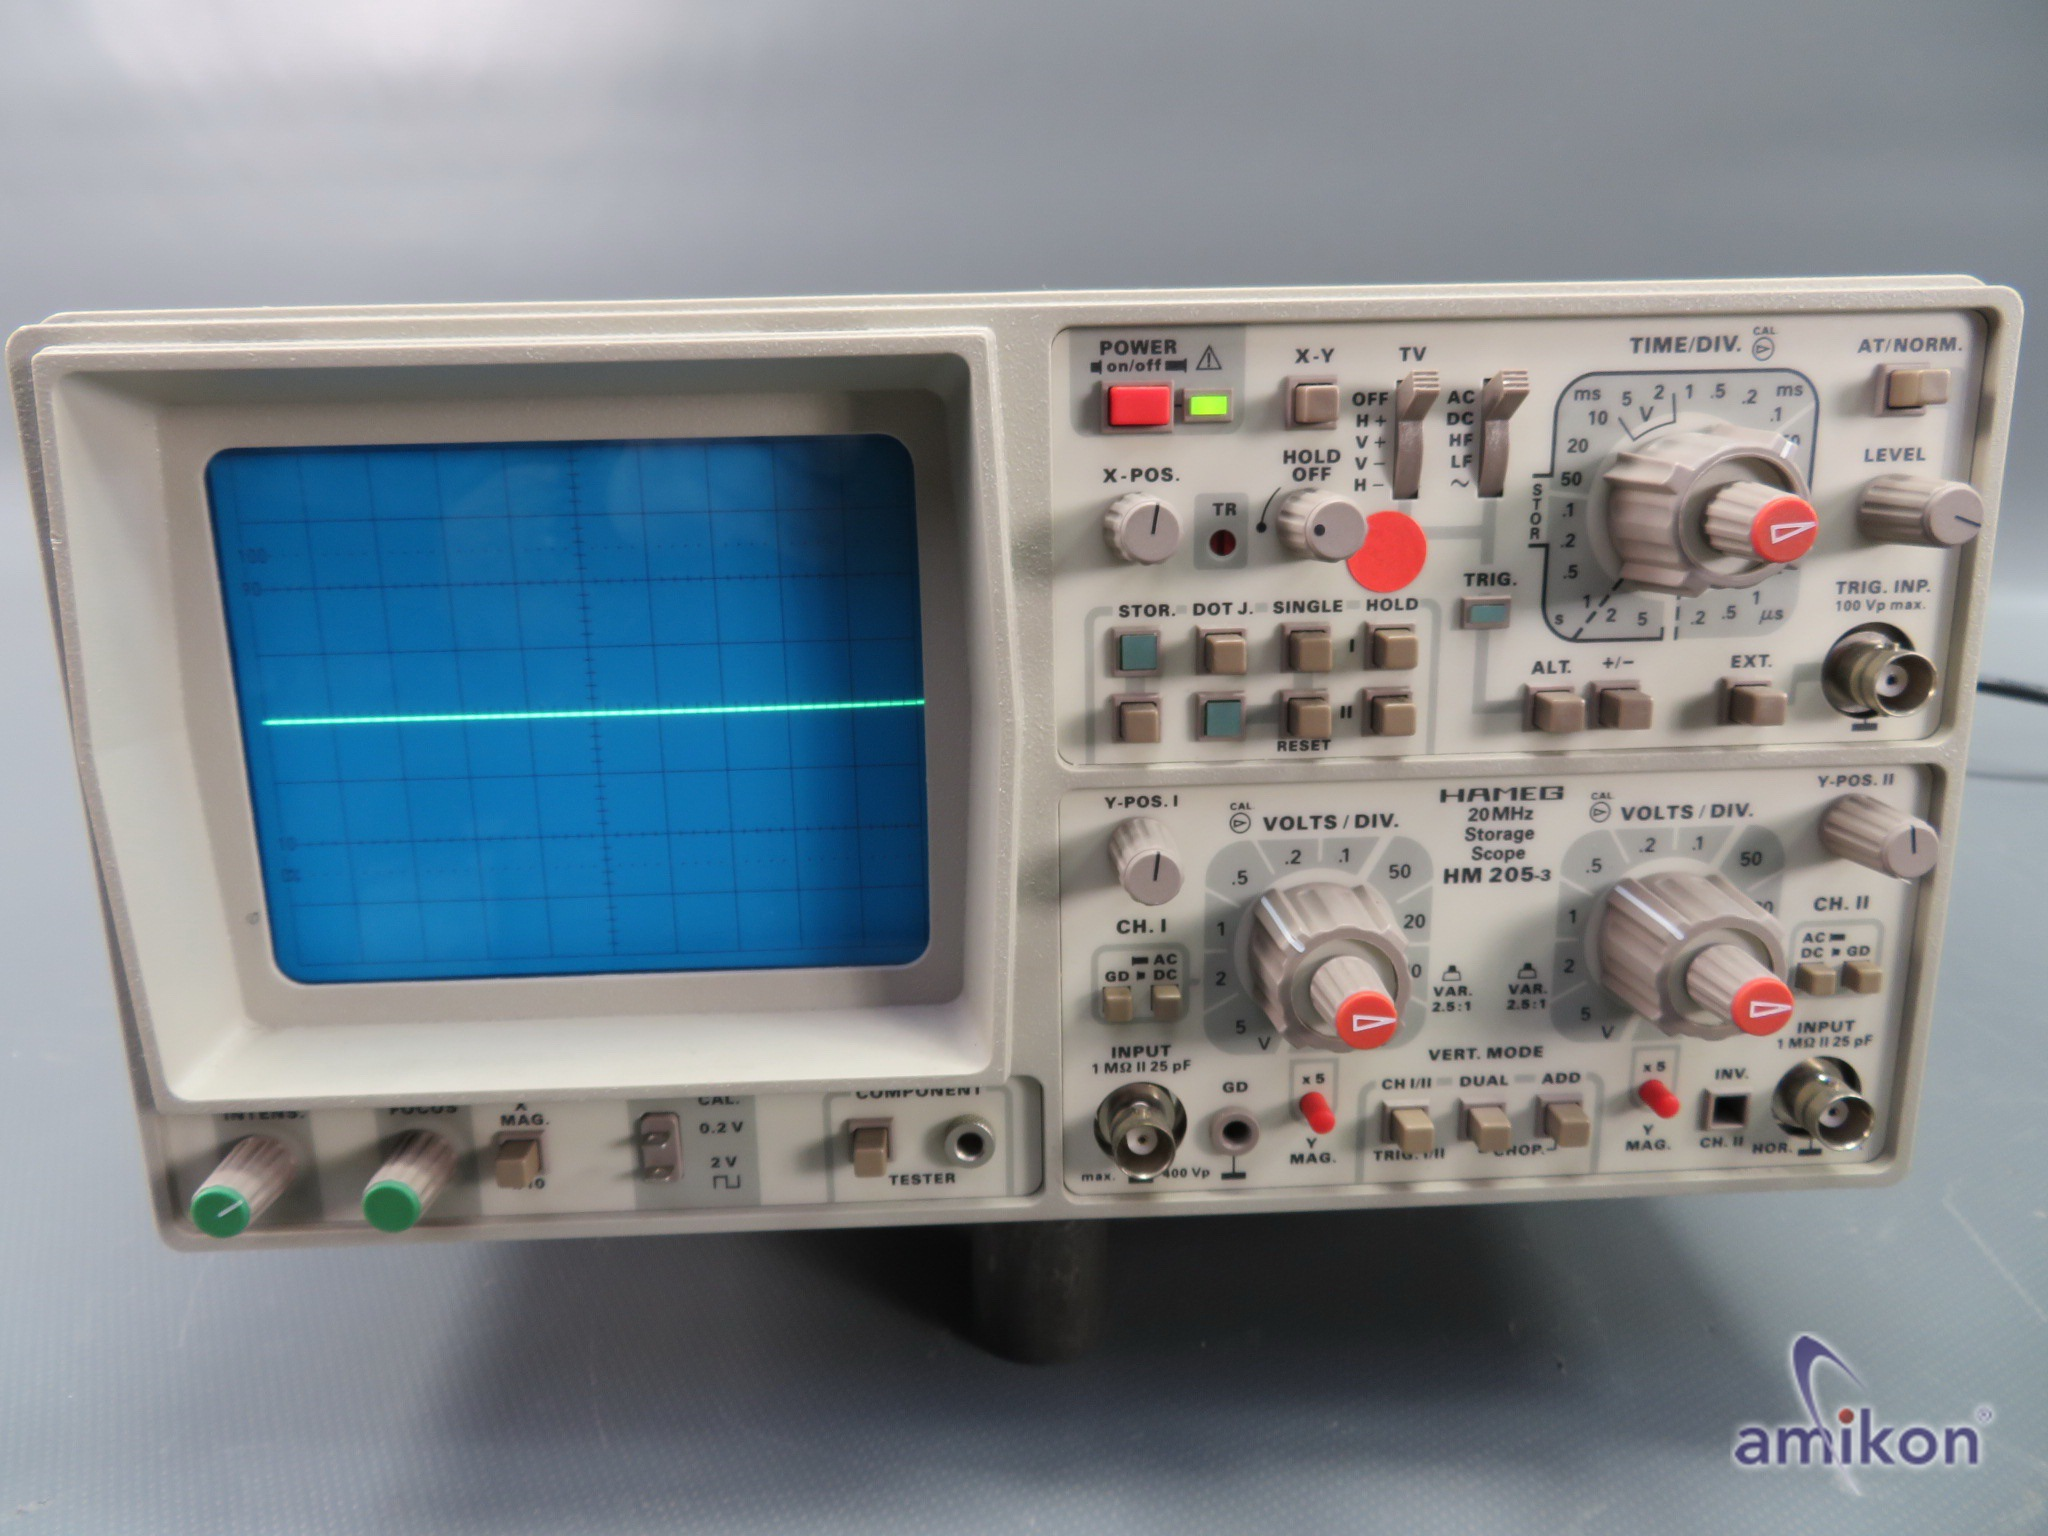
\includegraphics[width=\textwidth]{HAMEG-HM205-3.jpg}
        \caption{HAMEG Oszilloskop HM205-3\cite{Oszilloskop}}
        \label{fig:oszilloskop}
    \end{subfigure}
    \hfill
    \begin{subfigure}{0.45\textwidth}
        \centering
        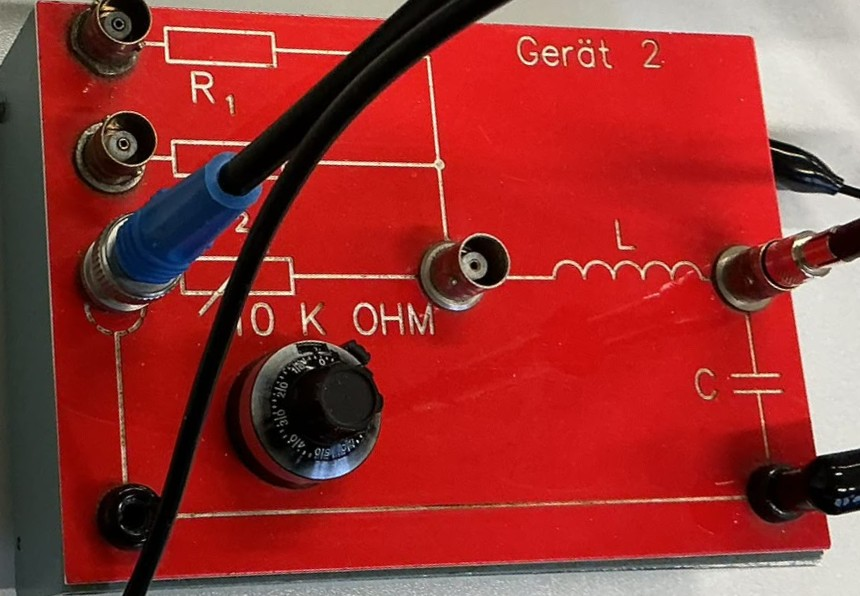
\includegraphics[width=\textwidth]{Geraet2.jpeg}
        \caption{Elektrischer Schwingkreis: Gerät 2 (eigene Aufnahme)}
        \label{fig:geraet2}
    \end{subfigure}
    \hfill
    \begin{subfigure}{0.45\textwidth}
        \centering
        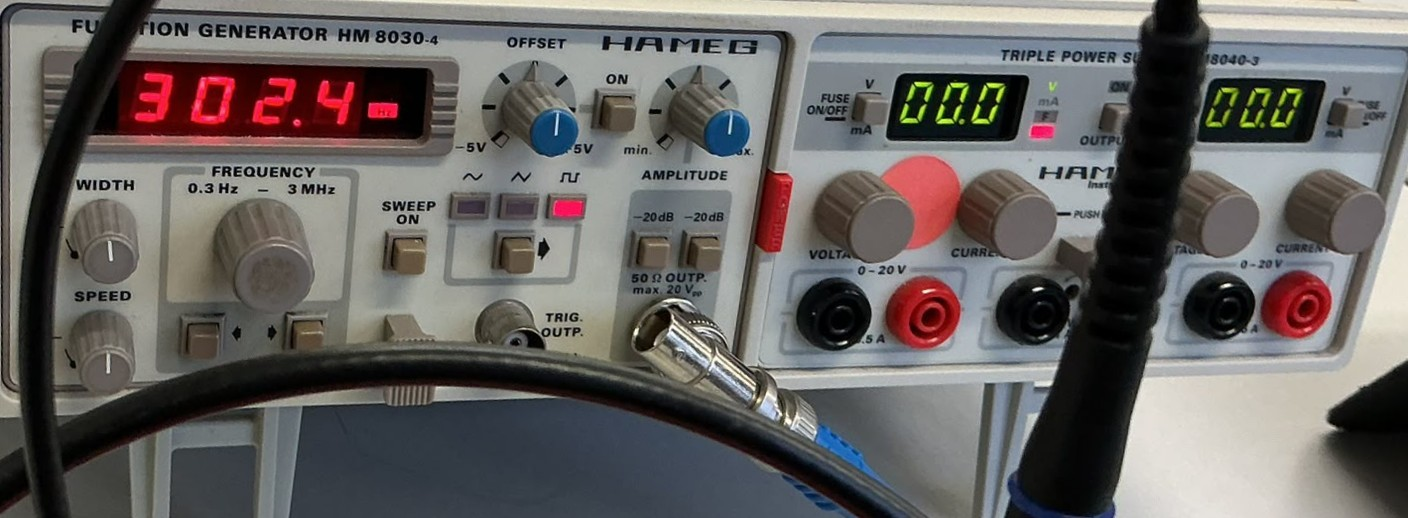
\includegraphics[width=\textwidth]{Frequenzgenerator.jpeg}
        \caption{Frequenzgenerator HAMEG HM8030-4 (eigene Aufnahme)}
        \label{fig:frequenzgenerator}
    \end{subfigure}
\end{figure}

\section{Durchführung}
Es werden in den folgenden Versuchen verschiedene Eigenschaften gedämpfter sowie erzwungener Schwingungen untersucht.
\subsection{Zeitabhängigkeit Amplitude}
Es wird zunächst die Zeitabhängigkeit der Schwingungsamplitude einer gedämpften Schwingung untersucht, um den kleineren der beiden Festwiderstände des Gerätes 2 zu bestimmen.
Dafür wird der Frequenzgenerator auf eine 302.4 Hz Sägezahnspannung eingestellt und an $R_1$ angeschlossen(\ref{fig:frequenzgenerator}). Der Tastkopf wird an den Abgriff nach der Spule $L$ und an den linken Input des Oszilloskops angeschlossen(\ref{fig:geraet2}). Für die Messung wird eine Einstellung des Oszilloskops von 0.2 V/DIV und 50$\mu$s/DIV gewählt und über die Peak-to-Peak Methode die Amplitude gemessen(\ref{fig:oszilloskop}).
\subsection{Aperiodischer Grenzfall}
In dieser Messung wird untersucht bei welchem Dämpfungswiderstand der Aperiodische Grenzfall eintritt. Dafür wird der vorherige Festwiderstand auf $R_1$ für den Regelbaren Widerstand ausgetauscht. Bei dem Oszilloskop wird die Einstellung 2$\mu$s/DIV gewählt(\ref{fig:oszilloskop}). Alle anderen Einstellungen werden nicht verändert. Der veränderbare Widerstand wird nun variiert, bis der aperiodische Grenzfall eintritt(\ref{fig:geraet2}).
Dies wird über zwei verschiedene Methoden bestimmt. Zunächst wird der Widerstand auf seinen Maximalwert eingestellt und dann langsam verringert, bis der aperiodische Grenzfall eintritt. Danach wird der Widerstand auf seinen Minimalwert eingestellt und langsam erhöht, bis der aperiodische Grenzfall eintritt. Die beiden Werte werden notiert und verglichen.
\subsection{Frequenzabhängigkeit Spannung und Phase}
Um die Frequenzabhängigkeit der Kondensator- und Erregerspannung sowie ihrem Phasenunterschied zu untersuchen, wird anstelle des einstellbaren Widerstandes der größere feste Widerstand $R_2$ eingesetzt(\ref{fig:geraet2}). Weiterhin wird der Trigger Output des Frequenzgenerators mit dem Trigger Input des Oszilloskops verbunden. Die Spannung des Frequenzgenerators wird außerdem direkt an den rechten Input des Oszilloskops angeschlossen und als Sinusspannung gewählt(\ref{fig:frequenzgenerator}).
Das Oszilloskop wird auf beiden Seiten auf 0.5 V/DIV und insgesamt auf 10$\mu$s/DIV eingestellt. Über den Dual Knopf werden beide Spannungen angezeigt(\ref{fig:oszilloskop}). 
Zunächst wird die Resonanzfrequenz bestimmt, indem die Frequenz des Frequenzgenerators variiert wird, bis die maximale Kondensatorspannung erreicht wird. Die Spannungen des Kondensators und des Erregers werden über die Peak-to-Peak Methode gemessen und notiert. Es wird der Phasenunterschied der beiden Spannungen über bestimmung des Zeitunterschieds zwischen den Peaks der Spannungen sowie der Periodendauer der Kondensatorspannung berechnet. Dieser Vorgang wird nun in zehn mal in 0.5 kHz Schritten jeweils nach unten und oben wiederholt, sowie bei 10 kHz, bei 20 kHz und bei 50 kHz(\ref{fig:frequenzgenerator}).